\section{Interest flooding mitigation methods}
\label{sec:design}

% Points what should be here:
% - What can be done (in general) to mitigate flooding attack
% - Which building blocks NDN architecture gives to mitigate Interest flooding attacks: Interest limits, ability to measure Interest satisfaction performance (Interest satisfaction stats)
% - Methods to set these limits: static/dynamic
% - Methods how limits can be applied: best-effort (fifo), "fair" queuing, probabilistic
% - Reference to caching: we don't consider it here, but caching provides additional level of protection, especially for certain types of attacks

% Our definition of attack mitigation is that good clients are still able to access data on the producer.

In this section we present several algorithms to mitigate Interest flooding attacks in NDN.  Our mitigation strategies feature varying degrees of implementation complexity and effectiveness---the higher the implementation complexity, the more effective is the algorithm against Interest flooding attacks. We start by describing our simple strategies and use the insights and lessons learnt from the deployment of these techniques to inform and design more effective mitigation techniques that can work well in a variety of attack scenarios.

%   - Naive approach to Interest Limits (that is called physical limits everywhere else)
%     Example how this can be implemented in a simple way
%     Baseline solution
%   - Interest limits with "fair" queuing
%     Improving problem of simple limits (no single face can dominate), but doesn't solve the proble

% - Attack mitigation
%   - Per-incoming interface Interest statistics

%   - Dynamic Interests limit adjustments

%   - Probabilistic Interest accept

%The fact that each Data packet takes the reverse path of the corresponding Interest packet allows intermediate routers to match a received Data packet to the corresponding Interest packet and %thus determine which Interest packets were satisfied. As we describe in the rest of this section,  NDN routers can exploit this information to make informed decisions on which Interest packets to %forward, how many Interest packets to forward, and thus effectively defend against DDoS attacks.

%Our methods to mitigate Interest flooding attack rely on the fundamental principle of the NDN architecture: the flow balance between Interest and Data packets: one Interest packet (the only communication initiator) can be satisfied with at most one Data packet.
%Because NDN is host-to-host architecture (as opposed to end-to-end in the current IP Internet), the flow balance principle allow any entity on the network, end-hosts and routers, control what and how much Data they want to receive.
%Therefore, any node can limit the number of forwarded Interests, effectively limiting the amount of the retrieved Data.
%At the same time, each forwarded Interest can be used to build up various data plane performance statistics, such as per-incoming interface ratios of satisfied Interests.

%\subsection{Na\"{i}ve attack mitigation}

%We start with a couple of naive strategies that can be used to migitate attacks in an NDN network and describe the pitfalls associated with these strategies.

% In a normal network operation, the size of Interests packets is supposed to be significantly smaller than the size of the requested Data.

% All communication in NDN network is host-to-host and receiver-driven.

An obvious and na\"ive solution to defend against Interest flooding attacks is to restrict the number of Interests that are forwarded in the network. To this end, we exploit a 
 fundamental principle of NDN architecture---flow balance between Interest and Data packets. The flow balance refers to the fact that one Interest can be satisfied by at most one Data packet. This principle allows intermediate routers that forward the Interest packets to control the number of outstanding Interests in the network. 
One simple and easy method to implement this strategy is for a NDN router to limit the number of forwarded Interests out of each interface based on the physical capacity of the corresponding out interface. This technique is a slight modification of the well-known {\it Token Bucket} algorithm that is currently widely used in packet switched networks. Analogous to the {\it Token Bucket} algorithm, NDN routers keep track of the amount of Data requested that can fully utilize the downstream link (estimated from the number of Interests it forwarded) and once the link capacity limit has been reached, they no longer forward new incoming Interests. Ideally, the number of tokens {\it i.e.} the \emph{Pending Interests Limit} for each link will be proportional to the link's bandwidth-delay product (BDP)~\cite{tcp-survey}. We can formalize this value as follows:
% With the objective to request as many Data packets, as downstream link can pump through, we are getting the following equation for Interest limit:

\begin{equation}
\mathrm{Interest\ Limit} = Delay\ [s] \cdot \frac{\mathrm{Bandwidth\ [Bytes/s]}}{\mathrm{Data\ packet\ size\ [Bytes]}}
\end{equation}

In the above equation, \emph{Delay} is the expected time of Interest being satisfied and \emph{Data packet size} is the size of the returned Data packet.
Although both these values are not known {\it apriori}, it is not really necessary to use their exact values.
One can simply set the pending Interest limit based on the average values of round trip time and observed Data packet size, as the network buffers can smooth out most of the network fluctuations.

This {\it Token Bucket} approach might be exceptionally retrictive in forwarding Interests -- not all Interests will result in a Data packet -- thus underutilizing the network. However, the biggest drawback of the algorithm is that it can be used as an effective mechanism to carry out denial of service attacks. If a router has utilized all its {\it tokens} to forward {\it bad} Interests on an out Interface, it can no longer forward incoming Interests from legitimate users on that out inteface till the pending {\it bad} Interests start to expire. One way to get around this issue is to impose a per-interface limit so that {\it bad} Interests are not allowed to entirely consume the limits of a specific interface. We describe this technique in greater detail below.

%That is, if it is known that the amount of already requested data ($=$~amount of forwarded Interests) can fully utilize the downstream link, an NDN node---either an end-user or an NDN router---has absolutely no point in forwarding new incoming Interests and creating corresponding PIT entries.
%For example, if a router A on Fig.~\ref{fig:flooding example} already forwarded 125 Interests requesting 1000-byte Data packets, any new incoming Interests can be almost safely dropped, provided the link capacity between A--B is 100~Mbps and delay is 10~ms.
%In other words, 125 Data packets returned by router B will fully utilize the link ($125 \times 1000 \mathrm{~bytes} \approx 10\mathrm{~ms} \times 100\mathrm{~Mbps}$) and any excess Data would be dropped.
%
%\subsubsection{\textbf{Interest limits (physical limits)}}
%\label{sec:physical limits}
%
%\subsection{Physical limits}
\label{sec:physical limits}

The requirement to send an Interest in order to receive Data packet, provides an NDN consumer a unique opportunity to request the right amount of Data.
Moreover, the same opportunity to control the amount of data flow is given not only to consumers, but all routers between consumer and producer (or nearby caches).  
In other words, every node, either a consumer or an intermediate router, is able to control how much data it wants to receive by limiting the number of forwarded Interests.

The limitation can implemented in a number of different ways, including leaky bucket scheduling and window-based flow control.
We decided to following TCP-like window-based flow control and applied the sliding window approach to implement Interest limits.

The size of the window defines how many Interests can be send out before Interests get satisfied or expired.
From the one hand, this size should be large enough to ``fill the pipe,'' meaning that a node needs to send enough Interests to receive Data at full capacity of the incoming link.
On the other hand, the window's size should not be too large to avoid excessive buffering and congestion of the Data packet.
Thus, the ideal size for such a window need to be defined proportional to link's bandwidth-delay product~\cite{tcp-survey}.
With the objective to request as many Data packets, as downstream link can pump through, we are getting the following equation for Interest limit:

\[
\mathrm{Interest\ Limit} = Delay\ [s] \cdot \frac{\mathrm{Bandwidth\ [Bytes/s]}}{\mathrm{Data\ packet\ size\ [Bytes]}}
\]

Note that the value of \textit{Delay} is not known a priory and varies between different Interest-Data flows.
However, we do not need to know the exact value of the delay and can set it as an average round trip delay among all flows (with a reasonable filtering of outliers).
This way, the statistical traffic multiplexing with link-level buffering will allow full utilization of the downstream link.
Exactly the same reasoning can be applied to the \textit{Data packet size} parameter, which can also be set to an average observed Data packet size.

Unlike rate-based approaches, window-based limiting does not require precise knowledge about the rate, as well does not need precise scheduling mechanisms.
Like in TCP, the window-based flow is self-clocking, easily adjusting itself to any traffic patterns.

%%% Local Variables: 
%%% mode: latex
%%% TeX-master: "../paper"
%%% End: 


%%%%%%%%%%%%%%%%%%%%%%%
%%%%%%%%%%%%%%%%%%%%%%%
%%%%%%%%%%%%%%%%%%%%%%%



\subsubsection{\textbf{Token bucket with per interface fairness}}
\label{sec:queuing}


% \subsection{Physical limits with ``fair'' queuing}
% \label{sec:queuing}

% However, this limitation approach does not attempt to utilize data plane performance knowledge (i.e., Interest satisfaction ratio statistics) to discriminate good and malicious Interests.

To partially overcome deficiencies of the Physical limits algorithm we need to ensure that the forwarded Interests represent at least a ``fair'' mix of the Interests received from different neighbors (interfaces).
That is, if the routers A on Fig.~\ref{fig:flooding example} has a very tight token budget, these tokens should be fairly distributed between incoming interfaces \texttt{eth0} and \texttt{eth1}.
Because of the very small volume of Interests, we cannot simply rely on network buffers to do statistical multiplexing of Interests, as they would almost never be buffered.
At the same time, until bag of tokens is not empty, there is no reason to delay Interest forwarding, as we do not known how many and from which interfaces Interests will arrive in the future.
Therefore, in order to achieve the goal of ``fair'' mixing of Interests, we need to implement additional mechanisms to buffer and mix incoming Interests, only if they cannot be immediately forwarded.

For the buffering part, we can reuse Pending Interest Table, with a small extension to support flagging of the Interests that cannot be forwarded immediately (see example on Fig.~\ref{fig:queueing}). 
As for the mixing part, we need an additional fair queuing mechanism, which can be implemented in a form of hierarchical queues (on Fig.~\ref{fig:queueing})\footnote{This essentially is a class based queuing, with classes for each outgoing/incoming interface.} or using virtual time approach~\cite{zhang1990virtual}. 
It should be noted that unlike normal queuing, Interest queues do not actually store a packet, but merely a bi-directional pointer to the existing PIT entry.
This way, PIT entry can be quickly updated when the Interest is actually forwarded, as well as the element can be removed from the queue when the Interest expires.

\begin{figure}[htbp]
  \centering
  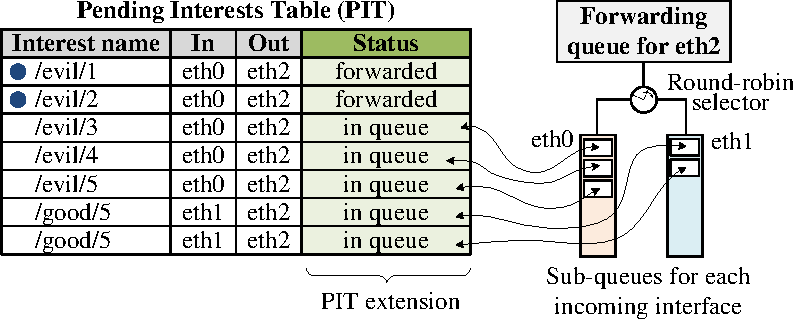
\includegraphics[scale=0.65]{queue}
  \caption{Interest queuing: if tokens are unavailable, the router creates PIT entry, but instead of forwarding, enqueued the Interest}
  \label{fig:queueing}
\end{figure}

A more formalized description of the Physical limits algorithms with per-interface fairness is presented in Pseudocode~\ref{alg:queuing}.
The algorithm extends the base Physical limits algorithm by enabling queuing when the bag of tokens is empty (lines 7--10), as well as by triggering an action (lines 16--21), when a token becomes available and enqueued Interest can be finally forwarded.
At the same time, the algorithm limits number of Interests allowed in a queue, constraining memory usage increase by at most a constant factor, compared to the base Physical limits algorithm (i.e., memory attack on routers are still unfeasible).


\floatname{algorithm}{Pseudocode}

%%%%%%%%%%%%%%%%%%%%%%%%%%%%%%
%%%%%%%%%%%%%%%%%%%%%%%%%%%%%%
%%%%%%%%%%%%%%%%%%%%%%%%%%%%%%

\begin{algorithm}[h]
\caption{Physical limits with per-interface fairness}
\label{alg:queuing}
\begin{algorithmic}[1]
\State{} \Comment{Same initialization, InData and Timeout functions as in Physical Limits algorithm}

\vspace{0.2cm}

\Function{OutInterest}{Interest \textbf{i}, InInterface \textbf{if}, OutInterface \textbf{of}}
    \If{$L_{of} - O_{of} > 0$} \Comment{\textbf{of} is under physical limits}
        \State $O_{of} \leftarrow O_{of} + 1$  \Comment{``Borrow'' token}
        \State add \textbf{of} to PIT entry and forward \textbf{i} to \textbf{of}
    \Else
        \State Queue $q \leftarrow of$.GetSubQueue($if$)
        \If{$Size(q) < L_{of}$}
           \State $q$.PushInterest($i$)
           \State add \textbf{of} to PIT entry, and link PIT entry with the queue
        \Else
           \State drop Interest
        \EndIf
    \EndIf
\EndFunction

\vspace{0.2cm}
\State{} \Comment{\textit{Whenever $L_{of} - O_{of}$ becomes larger than zero}}
\Function{TokenBecomesAvailable}{}
    \State Queue $q \leftarrow$ $of$.GetRoundRobinSubQueue 
    \State $i \leftarrow$ $q$.PopInterest
    \State update PIT entry and Forward($i$, $of$)
\EndFunction
\end{algorithmic}
\end{algorithm}


It should be noted that enqueued Interests should not be kept in the queue for a prolonged period of time.
Otherwise, by the time the Interests reaches the Data, the state could have been long expired downstream, effectively making such an Interest useless.
Additional mechanisms of pair-wise agreements between NDN routers and periodic Interest refresh can solve this particular problem, but it is out of the scope of the present paper.

As we show in Section~\ref{sec:evaluation}, fair queueing provides a partial relief from the Interest flooding attack, allowing legitimate users to successfully fetch Data for 15--20\% of the expressed Interests (compared to 0-10\% without fair queueing).
At the same time, the Physical limits with or without fair queueing allows attackers to send a relatively small volume of Interests in order to significantly impact service for the legitimate users.
Therefore, to successfully solve the problem, we need a more intelligent approach, allowing us to localize the attack traffic as close to the attack origin as possible.

%%% Local Variables: 
%%% mode: latex
%%% TeX-master: "../paper"
%%% End: 


%%%%%%%%%%%%%%%%%%%%%%%
%%%%%%%%%%%%%%%%%%%%%%%
%%%%%%%%%%%%%%%%%%%%%%%

The key drawback of the {\it Token Bucket} algorithm as well as its variation that ensures fair queuing on a per-interface basis is that these algorithms still admit Interests from malicious users. A sizeable percentage of these malicious Interests are forwarded all the way to content producers, thereby utilizing scarce network resources and reducing resources available to serve legitimate users.  These algorithms attempt to ensure that each interface does not forward more than its fair share of Interests, but in doing so, they drop both legitimate Interests as well as malicious Interests. For any strategy to be effective in defending against Interest flooding attacks, it must be able to detect and effectively drop only malicious requests for content. `Good' Interests from legitimate users must be admited and forwarded appropriately. The key question is how can we devise mitigation algorithms that allow a router to distinguish between `good' and `bad' Interests? 

Unlike in today's host-based Internet architecture where DDoS mitigation techniques that rely on blacklisting of dark IP prefixes or whitelisting of good IP prefixes are still reasonably effective, in NDN one cannot easily distinguish a `good' prefix from a `bad' one. Content producers must be able to support dynamic generation of Data packets to satisfy incoming Interest packets -- thus, an Interest that cannot be satisfied by matching Data from any intermediate router's cache is necessarily forwarded to the producer for possible dynamic Data packet generation. Thus intermediate routers cannot determine if the prefix is `good' or `bad' based on the name alone -- DDoS mitigation techniques that rely on whitelisting or blacklisting of certain namespaces  will be inefficient and likely ineffective. 

%%% Local Variables: 
%%% mode: latex
%%% TeX-master: "paper"
%%% End: 
